\documentclass{article}
\usepackage[a4paper, total={6in, 8in}]{geometry}
\usepackage{multicol,lipsum}
\usepackage[toc,page]{appendix}
\setcounter{secnumdepth}{3} 
\usepackage[english]{babel}
\usepackage[utf8x]{inputenc}
\usepackage[T1]{fontenc}


\usepackage{pdfpages}
\usepackage{xcolor}

\usepackage{graphicx}	        % Enable for eps and pdf figures, if they occur
\usepackage{hyperref}           % Enable embedded hyperlinks.
\usepackage{subcaption}
\usepackage{mwe}

\DeclareGraphicsExtensions{.pdf,.png,.jpg}
\usepackage{grffile} %per risolvere il problema di immagini con molti . prima dell'estensione
\hypersetup{
    colorlinks=true,
    linkcolor=blue,
    filecolor=magenta,      
    urlcolor=cyan,
}
 
\urlstyle{same}

\usepackage{listingsutf8}   		% Enable to use accent in Source code comment.
 \usepackage{listings}
 \usepackage{caption}
\usepackage{color}				% Eclipse style color
\definecolor{javared}{rgb}{0.6,0,0} % for strings

\lstdefinelanguage{JavaScript}{
  keywords={typeof, new, true, false, catch, function, return, null, catch, switch, var, if, in, while, do, else, case, break},
  keywordstyle=\color{blue}\bfseries,
  ndkeywords={class, export, boolean, throw, implements, import, this},
  ndkeywordstyle=\color{darkgray}\bfseries,
  identifierstyle=\color{black},
  sensitive=false,
  comment=[l]{//},
  morecomment=[s]{/*}{*/},
  commentstyle=\color{purple}\ttfamily,
  stringstyle=\color{red}\ttfamily,
  morestring=[b]',
  morestring=[b]"
}
\lstset{
   language=JavaScript,
  % backgroundcolor=\color{lightgray},
   extendedchars=true,
   basicstyle=\footnotesize\ttfamily,
   showstringspaces=false,
   showspaces=false,
   numbers=left,
   numberstyle=\footnotesize,
   numbersep=9pt,
   tabsize=2,
   breaklines=true,
   showtabs=false,
   frame = tb
}


\title{Web App Curricula - Ingegneria Informatica Unifi} % Article title
\author{Francesco Ermini}
\date{\today} % Leave empty to omit a date


\begin{document}
\maketitle

\newpage
\section{Introduzione}
Lo scopo di questo documento è quello di descrivere lo sviluppo della parte grafica del progetto webAppCurricula.
In particolare il documento è organizzato in tre sezioni:
\begin{enumerate}
\item Descrizione del linguaggio e dell'architettura usata ( \texttt{AngualarJS})
\item Panoramica su pagine, templates, controllers per la parte\emph{ Student}
\item Panoramica su pagine, templates, controllers per la parte \emph{Admin}
\end{enumerate}

\section{Sviluppo}
Il codice è raggruppato in due file:
\begin{itemize}
\item \emph{/client/index.html}
\item \emph{/client/admin/index.html}
\end{itemize}

\textbf{Attenzione:} la pagine amministratore non deve essere messa sul server perché al suo interno ci sono scritte le credenziali per poter accedere alle API che sono riservate all'amministratore. Si consiglia di tenere quella pagina in una cartella del computer ed aprirla come file sul browser.\\
Le librerie necessarie sono tutte incluse da CDN remoto (se non si è connessi a internet non funziona). Nella cartella css si trovano i fogli di stile. Nella cartella JS si trovano gli script necessarie a fare il download del PDF relativo al piano di studi.
\subsection{pagina, controller e template}
AngualarJS è stato organizzato secondo lo schema di cui si riporta un scheletro:
\begin{lstlisting}[caption = AngualrJS structure ]
<html>
<!-- Template -->
<script type="text/ng-template" id="/my_template.html">
	/* html code here */
</script>
<!-- Data Factory -->
<script>
angular.module('app', ['ngRoute']).factory('dataFactory', ['\$http', function(\$http) {
    dataFactory.getAPI = function () {
        /* API interfaces here */
        return \$http.get( 'http://localhost:5000/api/');
    };
<!-- Controller  -->
</script>
.controller('my_controller', ['$scope', 'dataFactory', function ($scope, dataFactory) {
    /* Business logic and html data binding here */
}])
<!-- Page -->
.config(function($routeProvider) {
    $routeProvider.when('/my_page', { /* page navigation here */
      templateUrl: '/my_template.html',
      controller: 'my_controller'
    })
\end{lstlisting}
%Quando il browser punta al link  \textit{index.html\/my\_page} viene fatto il render della pagina descritta in \emph{my\_template} ed eseguito il codice (in modo asimmetrico) in \emph{my\_controller}.

\newpage
\subsection{GUI Studente}

\begin{itemize}
\item \emph{\#/} : visualizzazione dei curricula e descrizione. Scelta di un curriculum.
\item \emph{\#/curriculum/<id>} : Scelta dei corsi e validazione del piano di studi sottomesso ( rispetto dei vincoli).
\item \emph{\#/studyplan/<id>} : Visualizzazione del piano di studi e download del pdf.
\item \emph{\#/student} : recupero del piano di studi tramite inserimento della matricola.
\end{itemize}

\begin{figure*}[!h]
        \centering
        \begin{subfigure}[b]{0.475\textwidth}
            \centering
            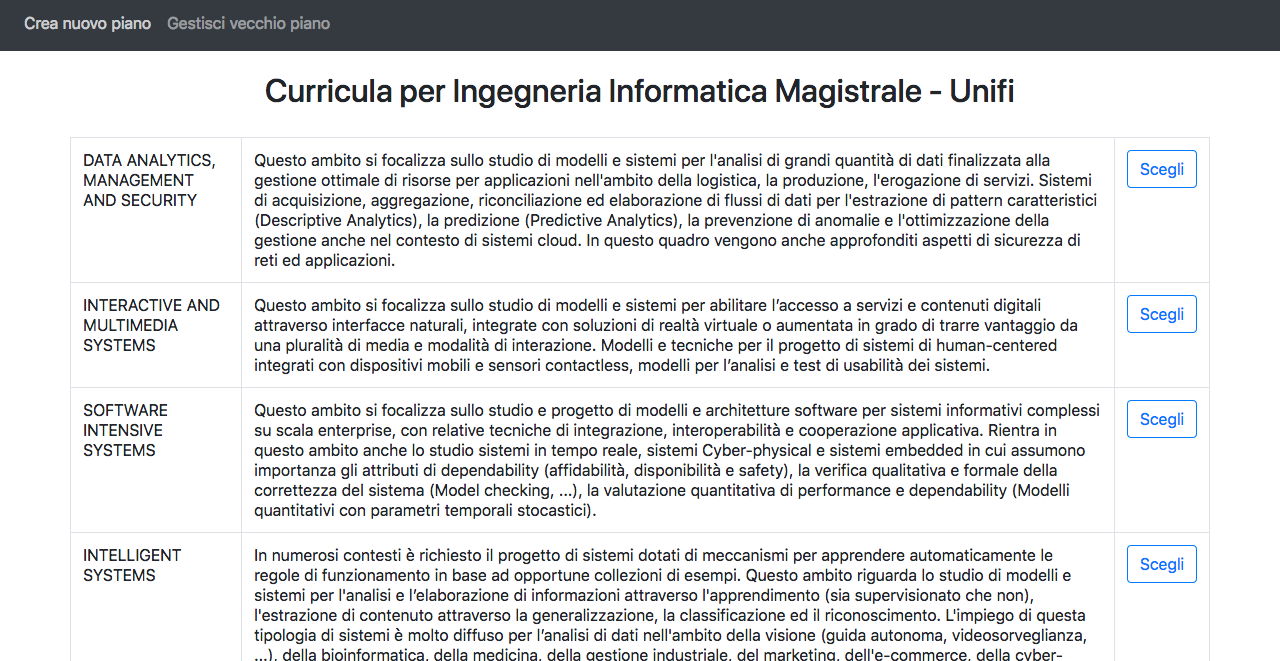
\includegraphics[width=\textwidth]{img/curricula.png}
            \caption[]%
            {{\small Scegli curriculum}}    
            \label{fig:Curricula}
        \end{subfigure}
        \hfill
        \begin{subfigure}[b]{0.475\textwidth}  
            \centering 
            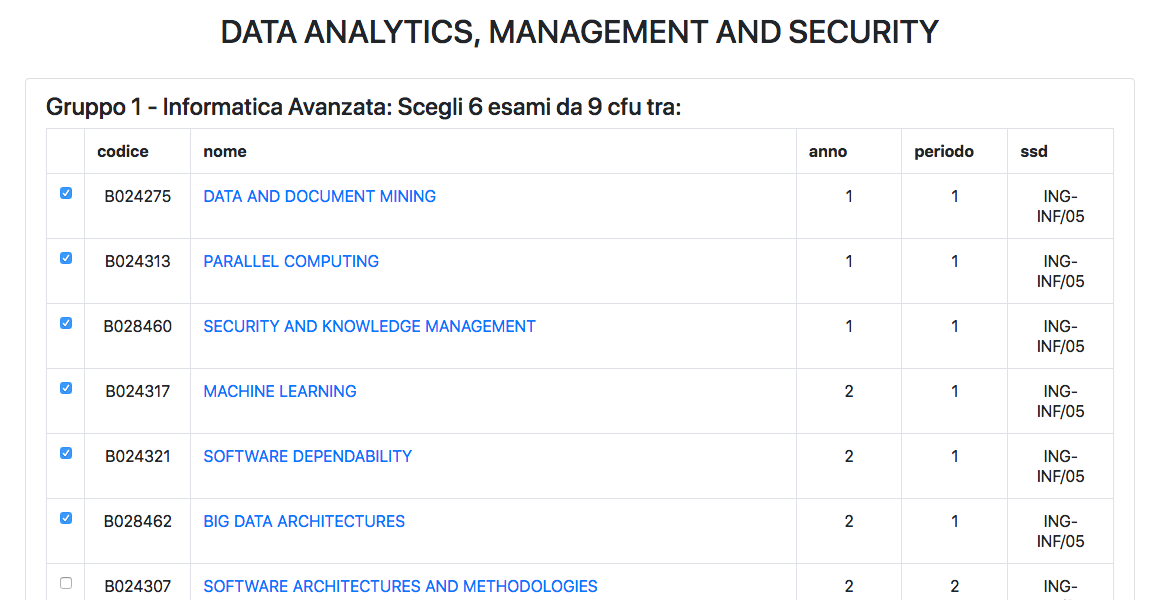
\includegraphics[width=\textwidth]{img/curriculum.png}
            \caption[]%
            {{\small Scegli corsi dal curriculum}}    
            \label{fig:Curriculum}
        \end{subfigure}
        \vskip\baselineskip
        \begin{subfigure}[b]{0.475\textwidth}   
            \centering 
            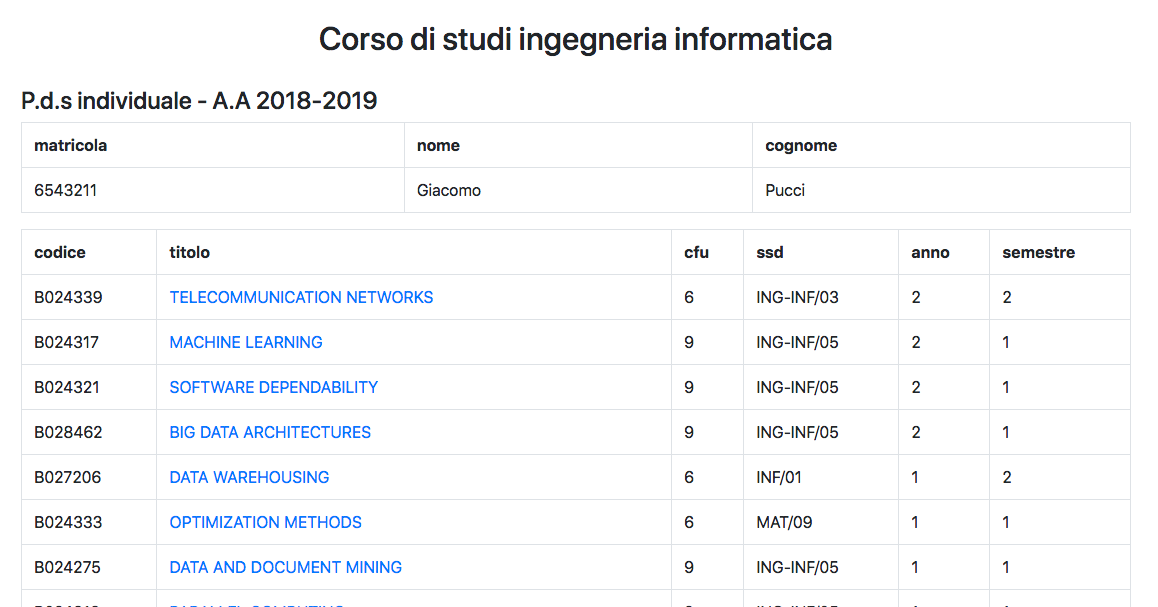
\includegraphics[width=\textwidth]{img/studyplan.png}
            \caption[]%
            {{\small Vedi piano di studi}}    
            \label{fig:Studyplan}
        \end{subfigure}
        \quad
        \begin{subfigure}[b]{0.475\textwidth}   
            \centering 
            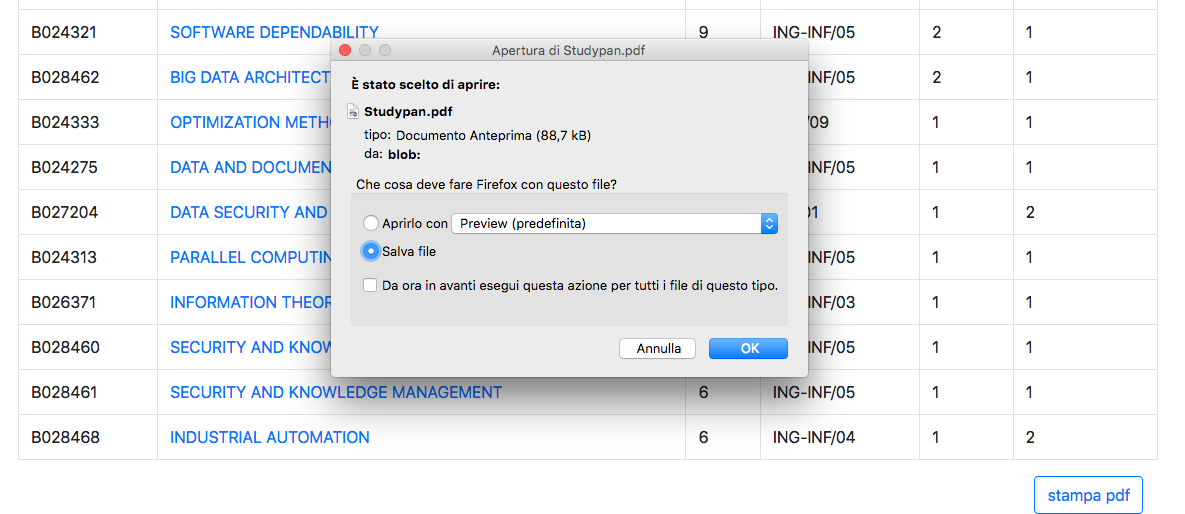
\includegraphics[width=\textwidth]{img/print.png}
            \caption[]%
            {{\small Scarica /stampa piano di studi }}    
            \label{fig:Print}
        \end{subfigure}
        \caption[  ]
        {\small GUI Studente} 
        \label{fig:Student GUI}
    \end{figure*}

\newpage
\subsection{GUI Admin}

\begin{itemize}
\item \emph{\#/} : Accesso rapido ai dettagli di un curriculum.
\item \emph{\#/curriculum} : Vista dell'elenco dei curricula. Accesso alle azioni CRUD per ogni curriculum.
\item \emph{\#/curriculum/create} : Inserimento dati per la creazione di nuovo curriculum (inclusa la scelta dei gruppi).
\item \emph{\#/curriculum/view/<id>} : Vista dei dati di uno specifico curriculum.
\item \emph{\#/curriculum/update/<id>} : Modifica dei dati di un curriculum esistente.
\item \emph{\#/group} : Vista dell'elenco dei gruppi. Accesso alle azioni CRUD per ogni gruppo.
\item \emph{\#/group/create} : Inserimento dei dati per la creazione di un nuovo gruppo (inclusa la scelta dei corsi).
\item \emph{\#/group/view/<id>} : Vista dei dati di un gruppo.
\item \emph{\#/group/update/<id>} : Modifica dei dati di un gruppo esistente.
\item \emph{\#/course} : Creazione, vista, modifica e cancellazione di un corso.
\item \emph{\#/academicyear} :  Creazione, vista, modifica e cancellazione di un anno accademico.
\end{itemize}


\begin{figure*}[!h]
        \centering
        \begin{subfigure}[b]{0.475\textwidth}
            \centering
            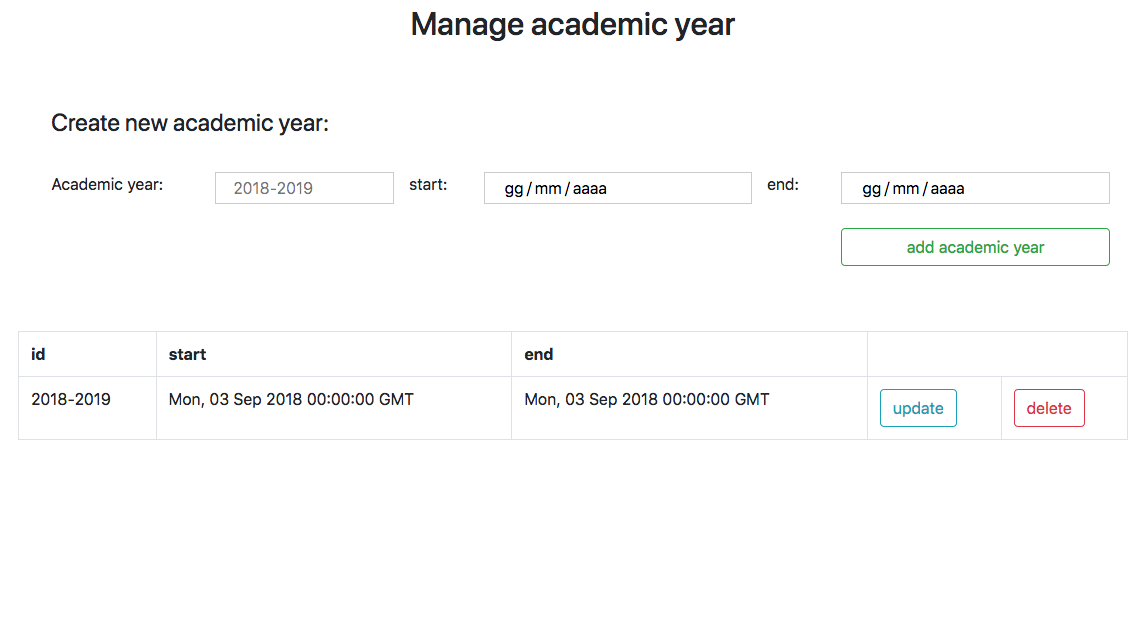
\includegraphics[width=\textwidth]{img/academicyearadmin.png}
            \caption[]%
            {{\small Gestisci anno accademico }}    
            \label{fig: Academic year management}
        \end{subfigure}
        \hfill
        \begin{subfigure}[b]{0.475\textwidth}  
            \centering 
            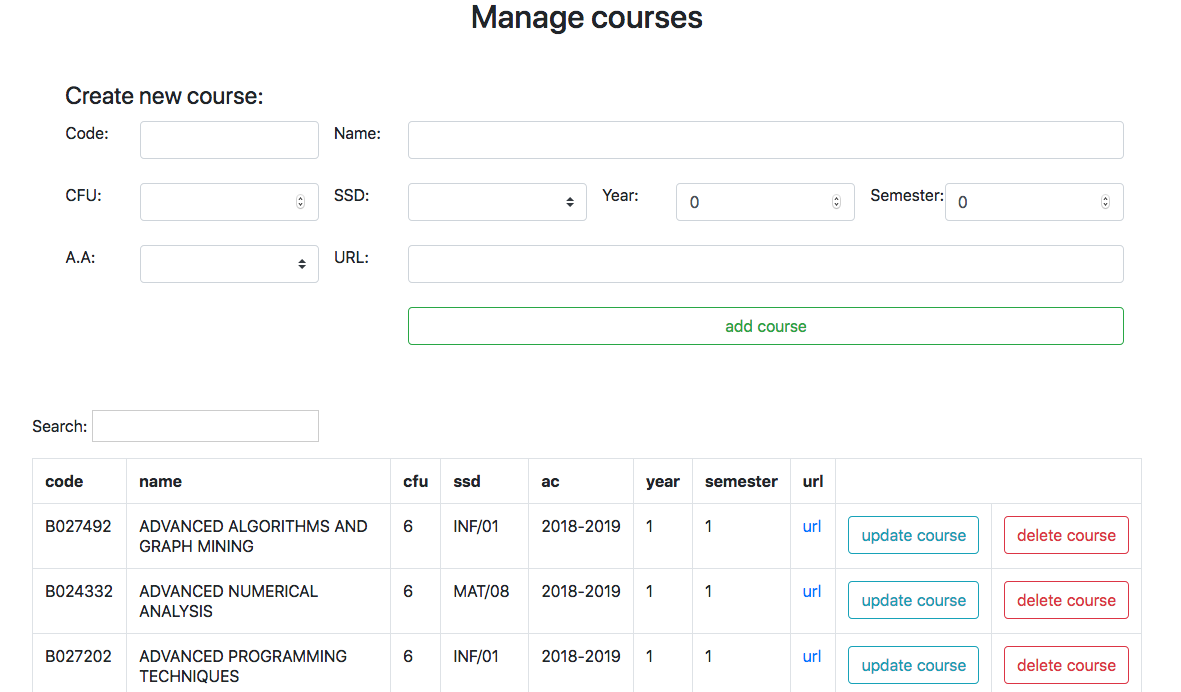
\includegraphics[width=\textwidth]{img/courseadmin.png}
            \caption[]%
            {{\small Gestisci corsi }}    
            \label{fig:Course Management}
        \end{subfigure}
        \vskip\baselineskip
        \begin{subfigure}[b]{0.475\textwidth}   
            \centering 
            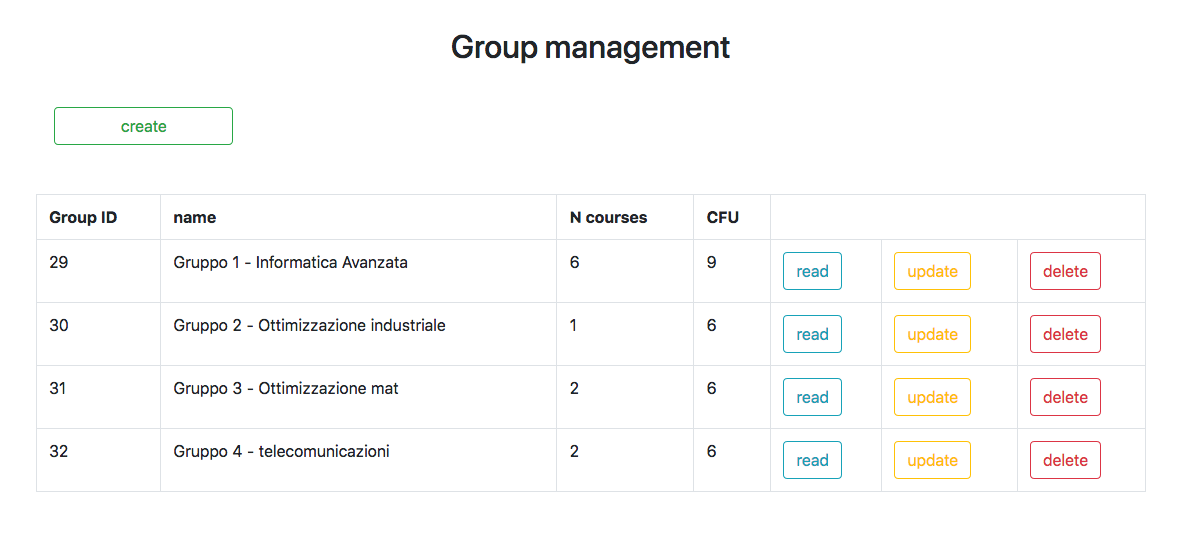
\includegraphics[width=\textwidth]{img/groupadmin.png}
            \caption[]%
            {{\small Gestisci gruppi }}    
            \label{fig:Group Management}
        \end{subfigure}
        \quad
        \begin{subfigure}[b]{0.475\textwidth}   
            \centering 
            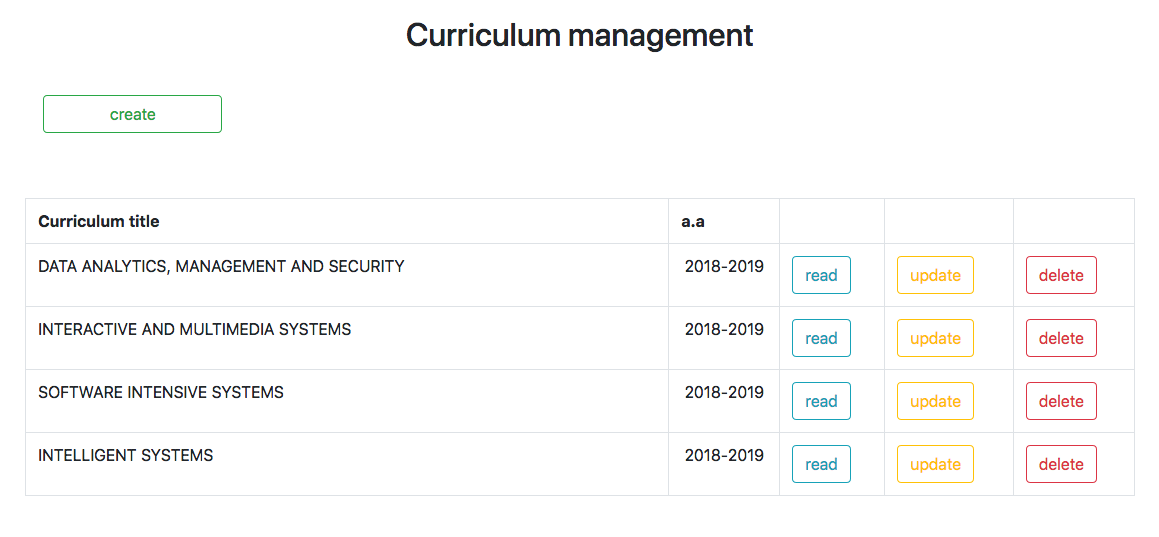
\includegraphics[width=\textwidth]{img/curriculumadmin.png}
            \caption[]%
            {{\small Gestisci Curricula }}    
            \label{fig:Curriculum Management}
        \end{subfigure}
        \caption[  ]
        {\small GUI Admin} 
        \label{fig:Student GUI}
    \end{figure*}


\newpage


\begin{thebibliography}{Bibliografia}
\bibitem{rif1}  Print PDF in AngualrJS \url{https://stackoverflow.com/questions/34049956/generate-pdf-from-html-using-pdfmake-in-angularjs}
\bibitem{rif2}  AngualrJS Facotory with API RESTful Serives \url{https://weblogs.asp.net/dwahlin/using-an-angularjs-factory-to-interact-with-a-restful-service}

\end{thebibliography}

\end{document}
